\newpage
\section{Resultados}

\subsection{Fonte de alimentação simétrica}
Após montar o circuito descrito pelo passo 1, obteve-se 6.04 V para Vdd e -5.98 V para Vss.


\subsection{Sensor de capacitivo}
Os dados obtidos para o sensor capacitivo, sendo a frequência de saída do oscilador em função da quantidade de água presente no recipiente, estão na tabela \ref{t_oscdata}.

\begin{small}
    \begin{table}[H]
        \begin{center}
            \caption{Frequência de saída do oscilador em relação a quantidade de água presente no recipiente do sensor capacitivo.}
            \begin{tabular}{l|l}
                \hline
                Água [mL] & Frequência [kHz] \\
                \hline
                55  & 2.689 \\
                \hline
                60  & 2.360 \\
                \hline
                65  & 2.090 \\
                \hline
                70  & 1.903 \\
                \hline
                75  & 1.728 \\
                \hline
                80  & 1.577 \\
                \hline
                85  & 1.489 \\
                \hline
                90  & 1.362 \\
                \hline
                95  & 1.246 \\
                \hline
                100 & 1.266 \\
                \hline
            \end{tabular}
            \label{t_oscdata}
        \end{center}
    \end{table}
\end{small}

A figura \ref{f_oscdata} mostra a curva do sensor, feita com os dados da tabela \ref{t_oscdata}.

\begin{figure}[H]
    \centering
    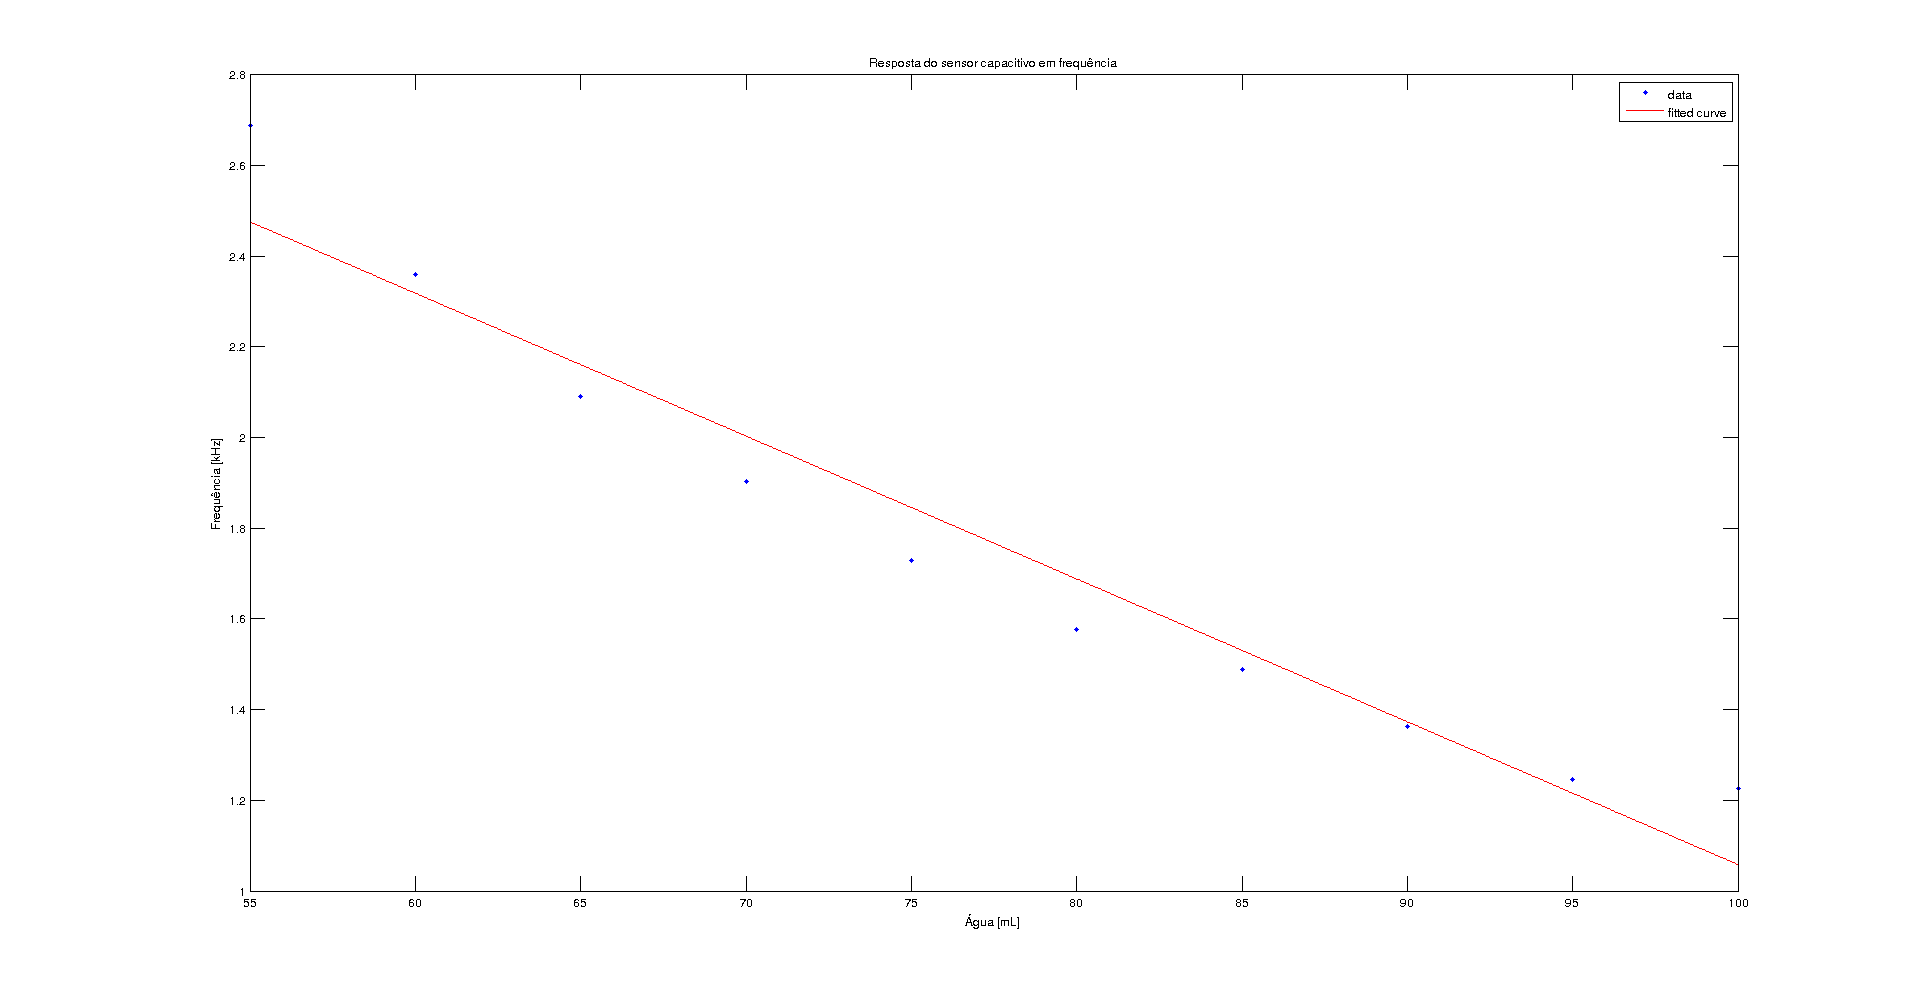
\includegraphics[scale=0.3]{img/oscdata.png}
    \caption{Curva característica do sensor com \textit{fit} polinomial de primeiro grau.}
    \label{f_oscdata}
\end{figure}

Com base no \textit{fit} polinomial de primeira ordem aplicado com o software MATLAB, foi possível obter a equação \ref{e_sensor}, onde $x$ é a quantidade de água em mililitros e $f(x)$ é a frequência em kHz, que descreve o comportamento do sensor. O erro quadrático médio para o \textit{fit} foi de 0.1222 kHz.

\begin{equation}
f(x) = -0.03151x + 4.209
\label{e_sensor}
\end{equation}